%%    TEMPLATE for articles submitted to the full-tex econf proceedings
%%     
%%
%%     Please do not remove lines commented out with %+
%%           these are for the editors' use.
%%
%%     Questions?  Send email to :  mpeskin@slac.stanford.edu
%%   

\documentclass[12pt]{article}
\usepackage{epsfig}
% \usepackage[document]{ragged2e}
\usepackage{siunitx, dirtytalk, hyperref, nicefrac, mathtools} 
\usepackage{graphicx,sectsty,longtable,tocloft,color,pdfpages,sidecap,subfig,array,eurosym}
 \captionsetup[figure]{labelfont={bf},name={Fig.},labelsep=period}

\usepackage{listings}
\usepackage{color}
\definecolor{codegreen}{rgb}{0,0.6,0}
\definecolor{codegray}{rgb}{0.5,0.5,0.5}
\definecolor{codepurple}{rgb}{0.58,0,0.82}
\definecolor{backcolour}{rgb}{0.95,0.95,0.92}
\lstdefinestyle{mystyle}{
    backgroundcolor=\color{backcolour},   
    commentstyle=\color{codegreen},
    keywordstyle=\color{magenta},
    numberstyle=\tiny\color{codegray},
    stringstyle=\color{codepurple},
    basicstyle=\footnotesize,
    breakatwhitespace=false,         
    breaklines=true,                 
    captionpos=b,                    
    keepspaces=true,                 
    numbers=left,                    
    numbersep=5pt,                  
    showspaces=false,                
    showstringspaces=false,
    showtabs=false,                  
    tabsize=2
}
\lstset{style=mystyle}

%%%%%%%%%%%%%%%%%%%%%%%%%%%%%%%%%%%%%%%%%%%%%%%%%%%%%%%%%%%%%%%%%%%%%%%%%%%%
%%  Do not change these:
\textwidth=6.0in  \textheight=8.25in

%%  Adjust these for your printer:
\leftmargin=-0.3in   \topmargin=-0.20in


%%%%%%%%%%%%%%%%%%%%%%%%%%%%%%%%%%%%%%%%%%%%%%%%%%%%%%%%%%%%%%%%%%%%%%%%%%%%
%  personal abbreviations and macros
%    the following package contains macros used in this document:
% \input LinksAndMetadata.tex
%%%%%%%%%%%%%%%%%%%%%%%%%%%%%%%%%%%%%%%%%%%%%%%%%%%%%%%%%%%%%%%%%%%%%%%%%%%
%
%  To include an item in the INDEX of the conference volume,
%           flag it with    \index{<item name>}
%  The use of this macro is illustrated in the text.
%
%%%%%%%%%%%%%%%%%%%%%%%%%%%%%%%%%%%%%%%%%%%%%%%%%%%%%%%%%%%%%%%%%%%%%%%%%%%%%

\def\Title#1{\begin{center} {\Large {\bf #1} } \end{center}}

\begin{document}


\Title{Manual: Internal tracker alignment for the g-2 experiment}

\bigskip\bigskip

%+\addtocontents{toc}{{\it D. Reggiano}}
%+\label{ReggianoStart}

\begin{raggedright}  
Gleb Lukicov$\,^{a}$\\
{\it $^{\mathrm{a}}$Department of Physics and Astronomy, University College London, London, \\ WC1E 6BT, United Kingdom}
\bigskip\bigskip
\end{raggedright}

\begin{center}
\today
\end{center}

\null\vspace{\fill}
\begin{abstract}
This document outlines the need for the internal alignment of the tracking detectors, and the methodology of the alignment. The software methods used in the alignment are summarised to allow for future alignment constants to be established for Run-3 and beyond. Internal alignment of the trackers in Run-1 and Run-2 has been established, with the constants defined as the interval of validity (IoV) in the reconstruction database. 
\end{abstract}
\vspace{\fill}

\tableofcontents

\clearpage

\section{Introduction}
In order for the tracking detector to reduce the systematic uncertainty on the $a_{\mu}$ measurement and improve the sensitivity to a muon EDM, a precise calibration of the tracking detector is required. One of such calibrations is the internal alignment, which considers the positions of the tracking modules within a station. 

Track-based internal alignment of the two stations of the tracking detector was implemented using data from Run-1 and Run-2. A Monte Carlo simulation was also developed to understand the detector geometry, and how the detector geometry affects how well the alignment can be determined, as well as to test the alignment procedure itself. A single figure-of-merit can really emphasise the need for a well aligned detector, as shown in Fig.~\ref{fig:rad_inter}, which highlights that even a relatively small scale of misalignment can have a large impact on the detector performance w.r.t to the beam extrapolation. Additionally, alignment is essential for setting a new limit on the muon EDM. Broadly speaking, an internal misalignment of an element of a tracking detector manifests as a presence of a large residual between a measurement (e.g. DCA of a hit to a wire) and a DCA of a fitted track to that wire. This large residual arises from the fact that the assumed detector position, which was used in the fitting of the track, is not the actual position of that detector. The aim of the alignment procedure is to establish the corrections to the assumed detector position, and hence, minimise the residuals.

\begin{figure}[h!]
\centering
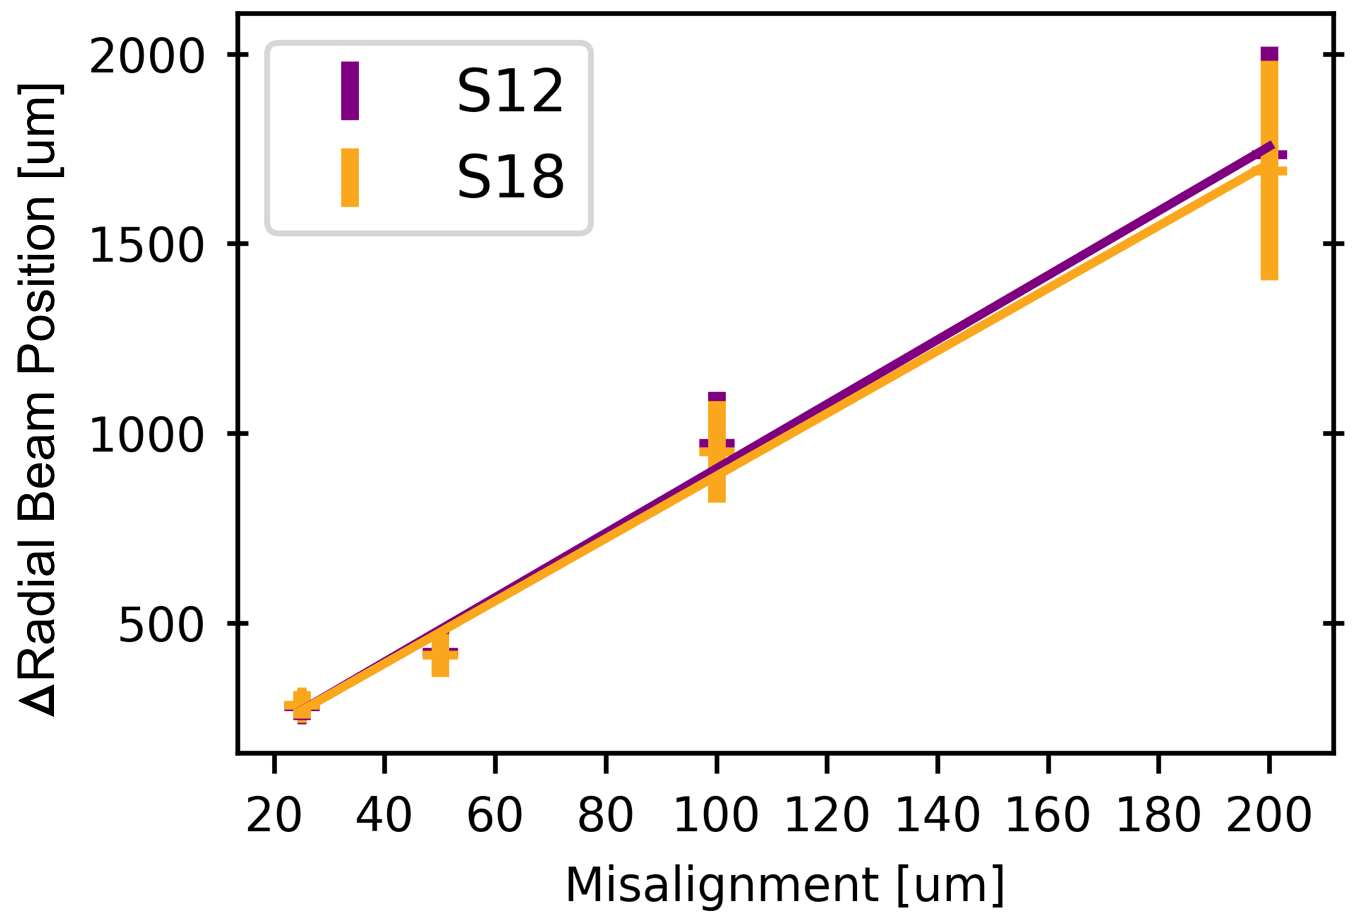
\includegraphics[width=0.6\linewidth]{fig/internal_rad.png}
\caption{Detector response to a uniform radial misalignment at different scales w.r.t to the difference in the extrapolated radial position.}
\label{fig:rad_inter}
\end{figure}

\section{Methodology of the alignment of the trackers}
he chosen alignment framework was \texttt{Millepede-II} \cite{mp2}, which utilises a simultaneous fit of many parameters describing the detector geometry and the input data. Under this method correlations between different alignment elements are taken into account, to produce an unbiased corrections to the position of the detector. The definition of the coordinate system used is shown in Fig~\ref{fig:Rotation}.

\begin{figure}[h!]
\centering
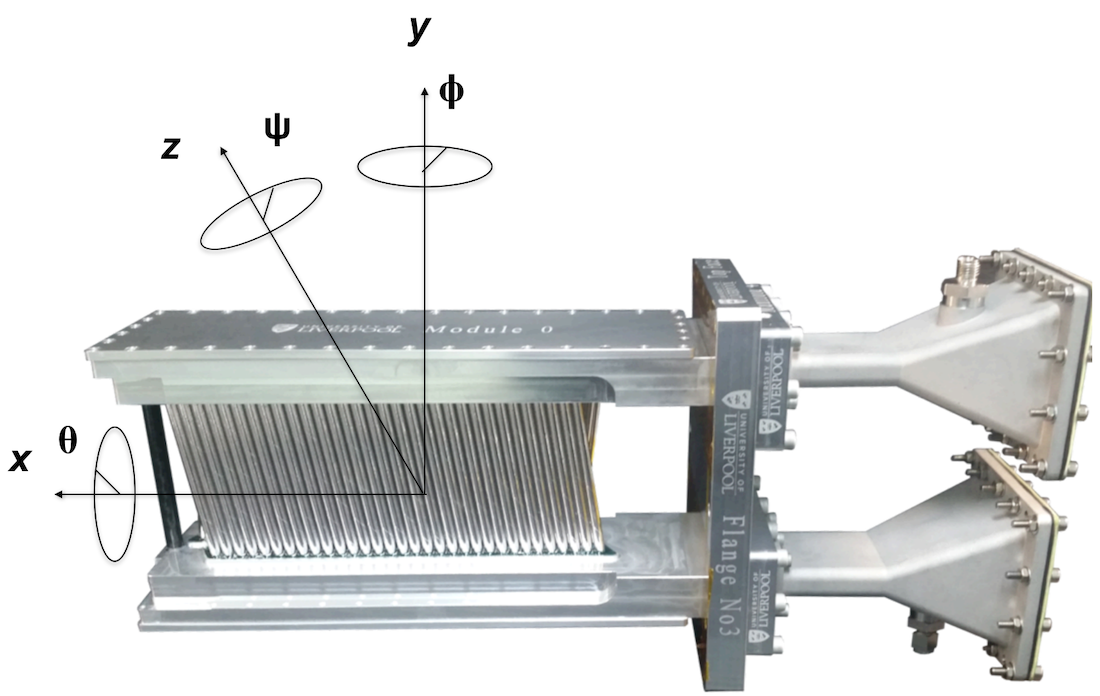
\includegraphics[width=0.6\linewidth]{fig/rotAxis.png}
\caption{Convention for misalignments (translations and rotation) in a module coordinate system. The radial and vertical shifts are along $x$ and $y$, respectively.}
\label{fig:Rotation}
\end{figure}

The alignment task can be summarised as a Least Squares Fit (LSF) problem with a very large number of parameters. These parameters can be divided into two classes: global and local parameters. Global parameters (i.e. the alignment parameters) affect all tracks (e.g. radial position of a detector). Local parameters are associated with individual fitted tracks. For example, a straight line fit in 2D will have 2 local parameters: a slope and an intercept. \texttt{Millepede-II} solves the linear LSF problem with a simultaneous fit of all global and local parameters minimising a linearised function of a sum of residuals. An objective function, $F$, is then minimised with respect to a variation of global and local parameters
\begin{equation}
\label{eq:obj_fun}
F(\boldsymbol{a},\boldsymbol{b})=\frac{\partial\chi^2(\boldsymbol{a},\boldsymbol{b})}{\partial(\boldsymbol{a},\boldsymbol{b})}=
\sum_{j}^{tracks}\sum_{i}^{hits} \frac{1}{(\sigma^{\mathrm{det}}_{i,j})^2} \frac{\big(r_{i,j}(\boldsymbol{a_0},\boldsymbol{b_0}_{,j})+\frac{\partial r_{i,j}}{\partial \boldsymbol{a}}
\delta \boldsymbol{a} +\frac{\partial r_{i,j}}{\partial \boldsymbol{b}_j}\delta \boldsymbol{b}_j\big)^2}{\partial(\boldsymbol{a},\boldsymbol{b})}=0,
\end{equation}
where $\boldsymbol{a_0}$ and $\boldsymbol{b_0}$ are the initially assumed geometry and track parameters, respectively, $r$ is the track residual (as shown in Fig.~\ref{fig:DriftCylinder}), and $\sigma^{\mathrm{det}}$ is the detector resolution. The corrections to the global parameters, $\delta\boldsymbol{a}$, allow for the minimisation of $F$, and are results of the alignment procedure. These corrections are then added to the assumed geometry of the detector to improve its performance.

\begin{figure}[tbp]
\centering
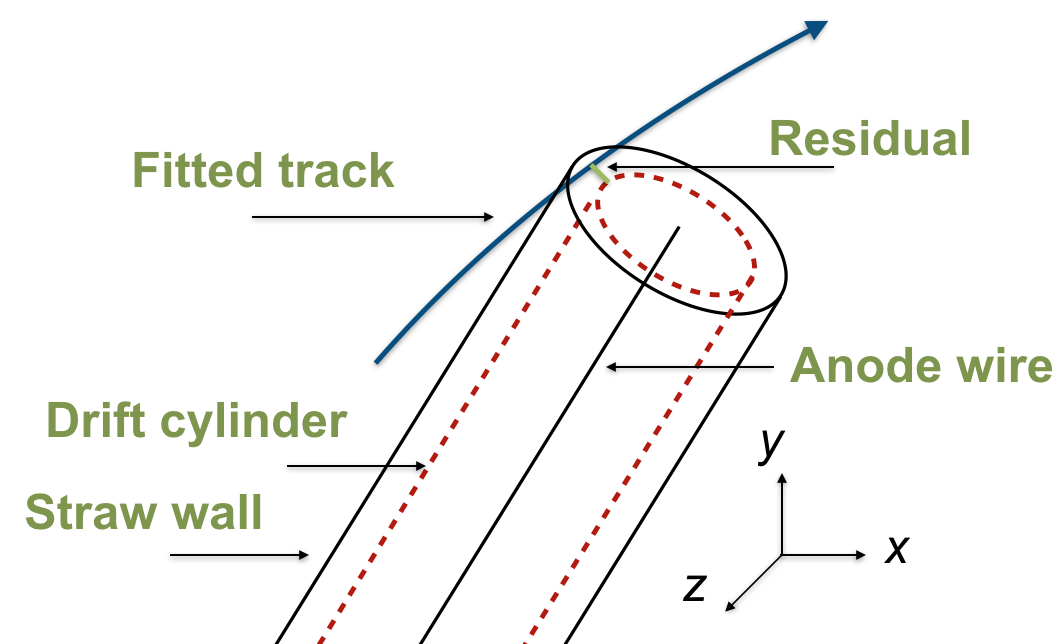
\includegraphics[scale = 0.45]{fig/DriftCylinder.png}  
    \caption{Visualisation of the drift cylinder, which is defined by the measured drift time in the straw.}
\label{fig:DriftCylinder} 
\end{figure}

\section{Alignment results}
In simulation (MDC1), alignment stability was reached stability, and alignment convergence within \SI{2}{\micro\metre} and \SI{10}{\micro\metre} radially and vertically, respectively, was established as shown in \textbf{\href{https://gm2-docdb.fnal.gov/cgi-bin/private/ShowDocument?docid=17551}{DocDB:17551}}. Stable alignment results and improved residuals in data, using run 15922, were reached as shown in \textbf{\href{https://gm2-docdb.fnal.gov/cgi-bin/private/ShowDocument?docid=17722}{DocDB:17722}}.

Stability of the alignment constants across 3 IoV of Run-1 and Run-2 are shown in \textbf{\href{https://gm2-docdb.fnal.gov/cgi-bin/private/ShowDocument?docid=AAAA}{DocDB:AAAA}}.

More detailed description of the alignment methods is contained in \textbf{\href{https://gm2-docdb.fnal.gov/cgi-bin/private/ShowDocument?docid=15106}{DocDB:15106}} (see backup also). While the uncertainty on the beam extrapolation due to the misalignment was estimated in \textbf{\href{https://gm2-docdb.fnal.gov/cgi-bin/private/ShowDocument?docid=16685}{DocDB:16685}}. 

\section{Software Methods}
The alignment software is part of the \verb!gm2tracker! project: \verb!gm2tracker/align/!. An alignment software module has been developed as part of the \textit{gm2 art} software framework. This module comes last in the tracking chain, taking the final track-data product (\verb!TrackArtRecords_tracks!) from either data or simulation. The geometry is fully described at the tracking stage and is passed to the alignment module, which also calculates the residuals of the selected tracks, as well as computes the local and global derivatives. A \verb!C++! infrastructure (\texttt{Mille}) is provided \cite{mp2} to write this information into a binary file which is passed to \texttt{PEDE} (a \texttt{Fortran} executable), which performs a simultaneous fit via a matrix inversion described above. The alignment module is also responsible for writing a constraints file (specifying the redundant degrees of freedom), and a steering file (specifying the mathematical methods used by \texttt{PEDE}). The final outputs of the \texttt{PEDE} algorithm are labels and the corresponding fitted values of the global parameters and their errors, if applicable. This algorithm is shown in Fig.~\ref{fig:mp2}.\\
\begin{figure}[tbp]
    \centering
    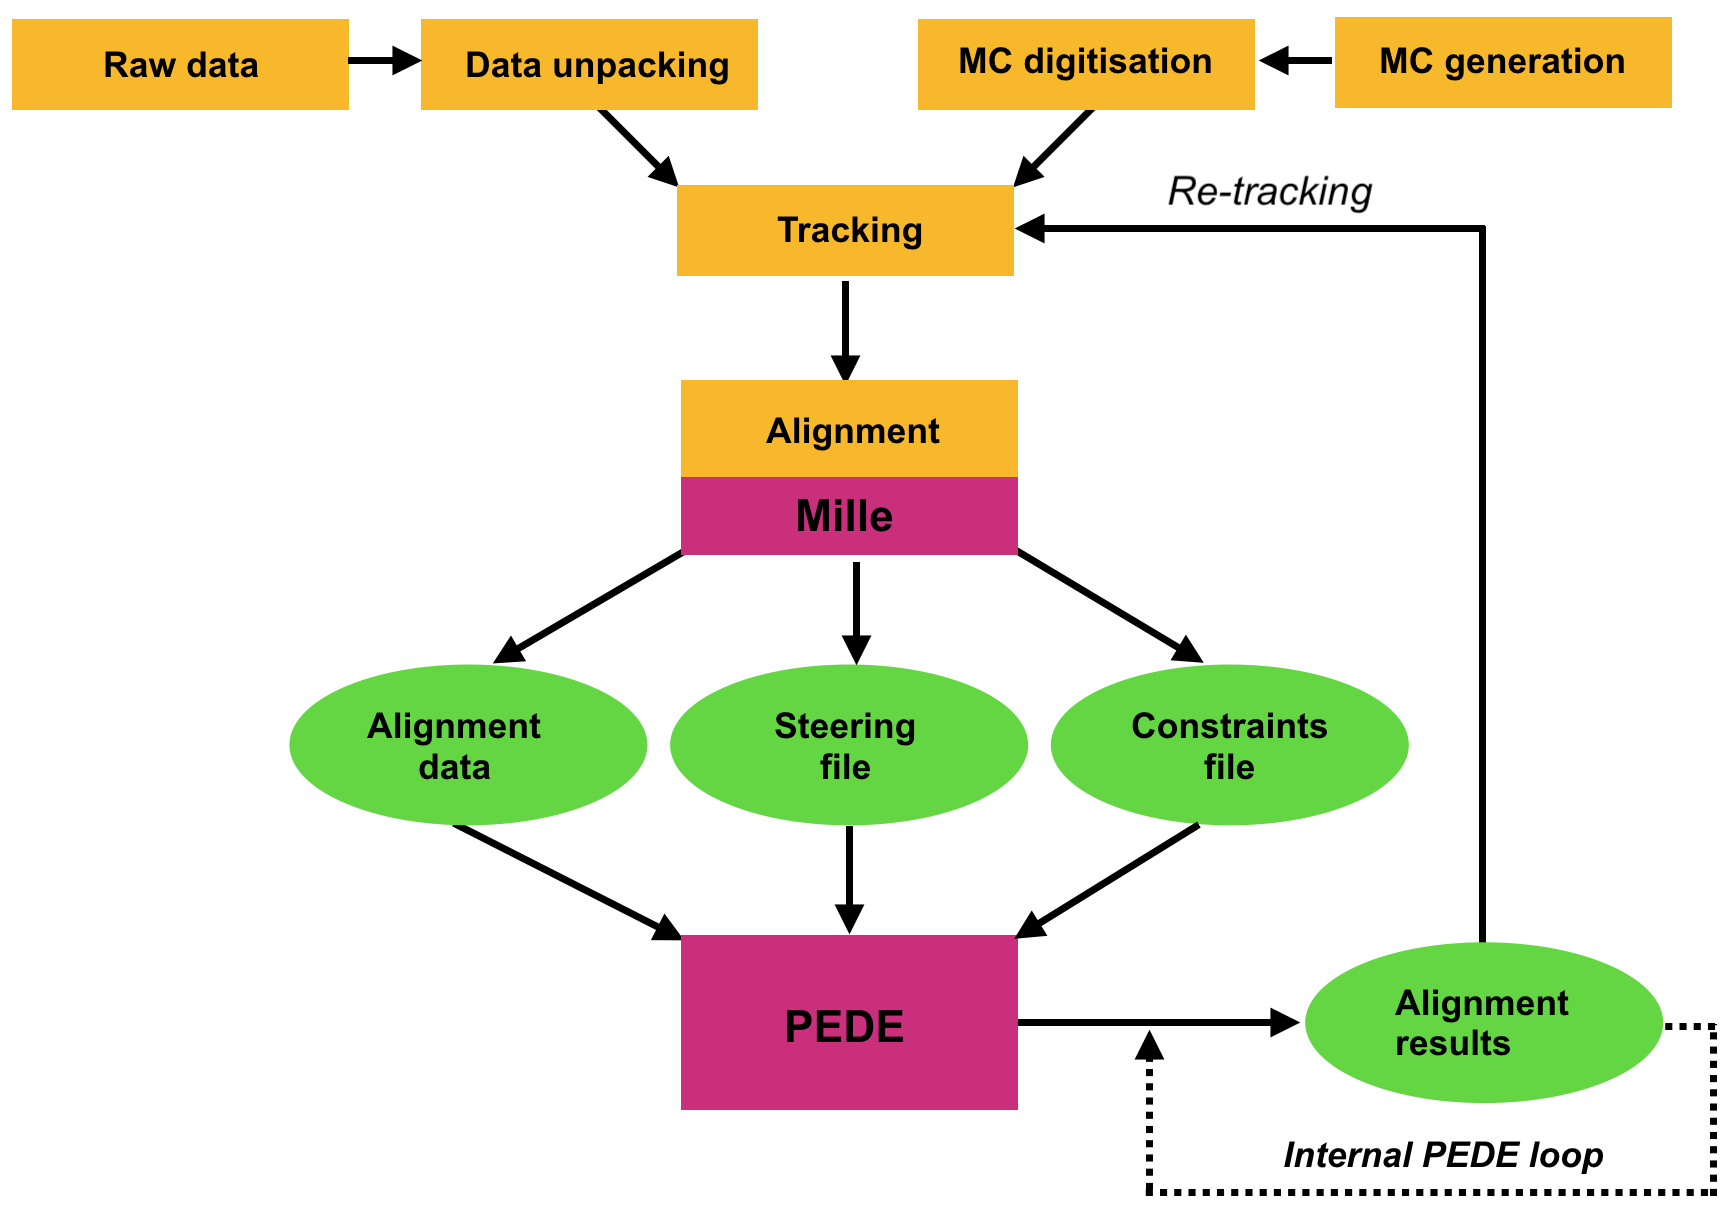
\includegraphics[scale = 0.44]{fig/MP2.png}
    \caption{The schematic of the \texttt{Mille} routine (shown in purple) with the \textit{gm2 art} software framework (shown in orange). The final result of alignment is then used in tracking to improve the residuals.}
    \label{fig:mp2}
\end{figure}

The steering file is
\lstinputlisting[language=Bash]{Steer.sh}

\subsection{Run iterative internal alignment on a single run with residual verification}

Commands and plots 

\subsection{Run internal alignment monitoring}
Commands and plots 
\subsection{Run internal alignment to establish constants for a run interval}
Commands and plots 

\section{Alignment constants and the reconstruction database}
The alignment constants will now used in the $gm2geom$ from the next release: $v9_28_00$ or $v9_27_01$, Once DB methods are established, the alignment constants will migrate to the IoV table. 

\begin{thebibliography}{99}

\bibitem{mp2} V. Blobel \textit{Software Alignment for Tracking Detectors}, Nucl. Instrum. Methods A, \textbf{556}, 5 (2006).

\end{thebibliography}

\def\Acknowledgements{
\setlength{\parskip}{0.3cm}\setlength{\parindent}{0.0cm}
     \bigskip\bigskip      {\Large {\bf Acknowledgements}} \bigskip}
\def\speaker#1{{\bf #1:}\ }
\def\endAcknowledgements{}

\Acknowledgements \\
I would like to thank the entire tracker group for their immense support in this project! In particular, I would like to express gratitude to Mark, Becky, James, Joe, Brendan, Saskia, Tammy and Nick for their advice.
\endAcknowledgements
 
\end{document}

